\documentclass[14pt,a4paper] {article}
\usepackage{mathtext}
\usepackage[T1,T2A]{fontenc}
\usepackage[utf8]{inputenc}
\usepackage[english]{babel}
\usepackage{extsizes}
\usepackage{cmap}

\usepackage{authblk}
\renewcommand\Affilfont{\itshape\small}
\renewcommand\Authands{, }

\usepackage{cite}
\usepackage{underscore}


\usepackage[pdftex]{graphicx}
\graphicspath{{imgs/}}


\usepackage{caption}

\renewcommand{\baselinestretch}{1.5}
%\frenchspacing

\usepackage{indentfirst}

\usepackage{geometry}
\geometry{left=2cm}
\geometry{right=1cm}
\geometry{top=1.5cm}
\geometry{bottom=1.5cm}


\begin{document}

\title{Handbook of Time-Resolved Scanning Kerr Microscopy in G31a}

\author{F.B. Mushenok, C.S. Davies, V.V. Kruglyak} 
\date{\today}
\pagenumbering{arabic}
\maketitle

\section{Introduction}
 The purpose of this manual is to collect and organize the best practices of measurement with Time-Resolved Scanning Kerr Microscopy setup in G31. Some parts of the manual were copied from manual of Carl Davies.
  Please, fill free to amend and improve the manual (if you are confident in what are you doing).
  
  F. Mushenok (mushenokf@gmail.com)  

\section{Laser safety}
  Before any experimental work in the lab, you should be familiar with laser safety rules. Please adhere to the best practise rules:
   
   
\section{Cold start}

\section{Preliminary work}

The laser system is maintained at a constant temperature, of 18 degrees celsius, by a coolant. This should always be kept on. 
First of all, inspect floor, area around the laser and bench surface for water leaks. If there are any water droplets or spillages, find the reason and amend it. Keep in mind potential danger of water spillage.

If the chiller is off, then press the buttion and switch it on, wait a couple of minutes and make sure make sure the chiller's display indicates 18 degree.  If the display inducates "ADD", then fill a canister with distilled water, open the large black cap (labelled (A) in Figure 1.1), and refill the coolant until the display reverts back to '18'.
\begin{figure}
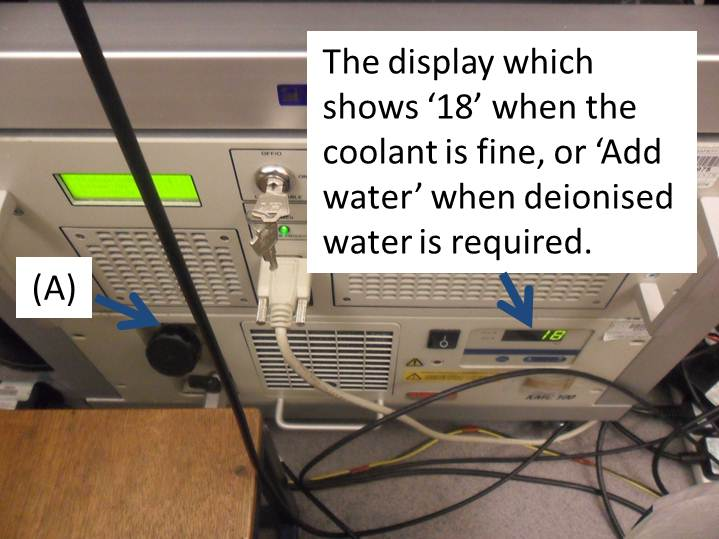
\includegraphics[width=0.5\linewidth]{Laser-coolant.jpg}
\caption{The front panel of the laser coolant}
\end{figure}

IMPORTANT!!! Every six months the water filter (on the rear side of the chiller) should be replaced on the new one.

\subsection{Mounting the sample}

The structure we wish to study lies on a substrate. Typical examples include a permalloy structure mounted on a silicon substrate, or a GaAs structure mounted on a glass substrate. The structure must first be attached to the printed circuit board ({\it PCB}), and to do this, we simply apply sticky-tape. Wearing latex gloves, and preferably with the help of a magnifying glass/angled lamp, the structure should be laid on top of the signal line of the PCB (the PCB consists of ground(yellow)-signal-ground(yellow) lines. The substrate should also be lying fully on the PCB. Care should be taken to ensure this is done correctly - in my personal experience, it has sometimes taken up to an hour to do this.
\\

A good way to double-check this step has been done correctly is to take a photo of the sample (where you can see it), and then a second photo of the sample lying on the PCB (scratches on the PCB invariably make the structure on the substrate impossible to discern). Using an application as simple as Microsoft Powerpoint gives us a way to verify that the structure is lying on the signal line (see Figure 2) 

\begin{figure}
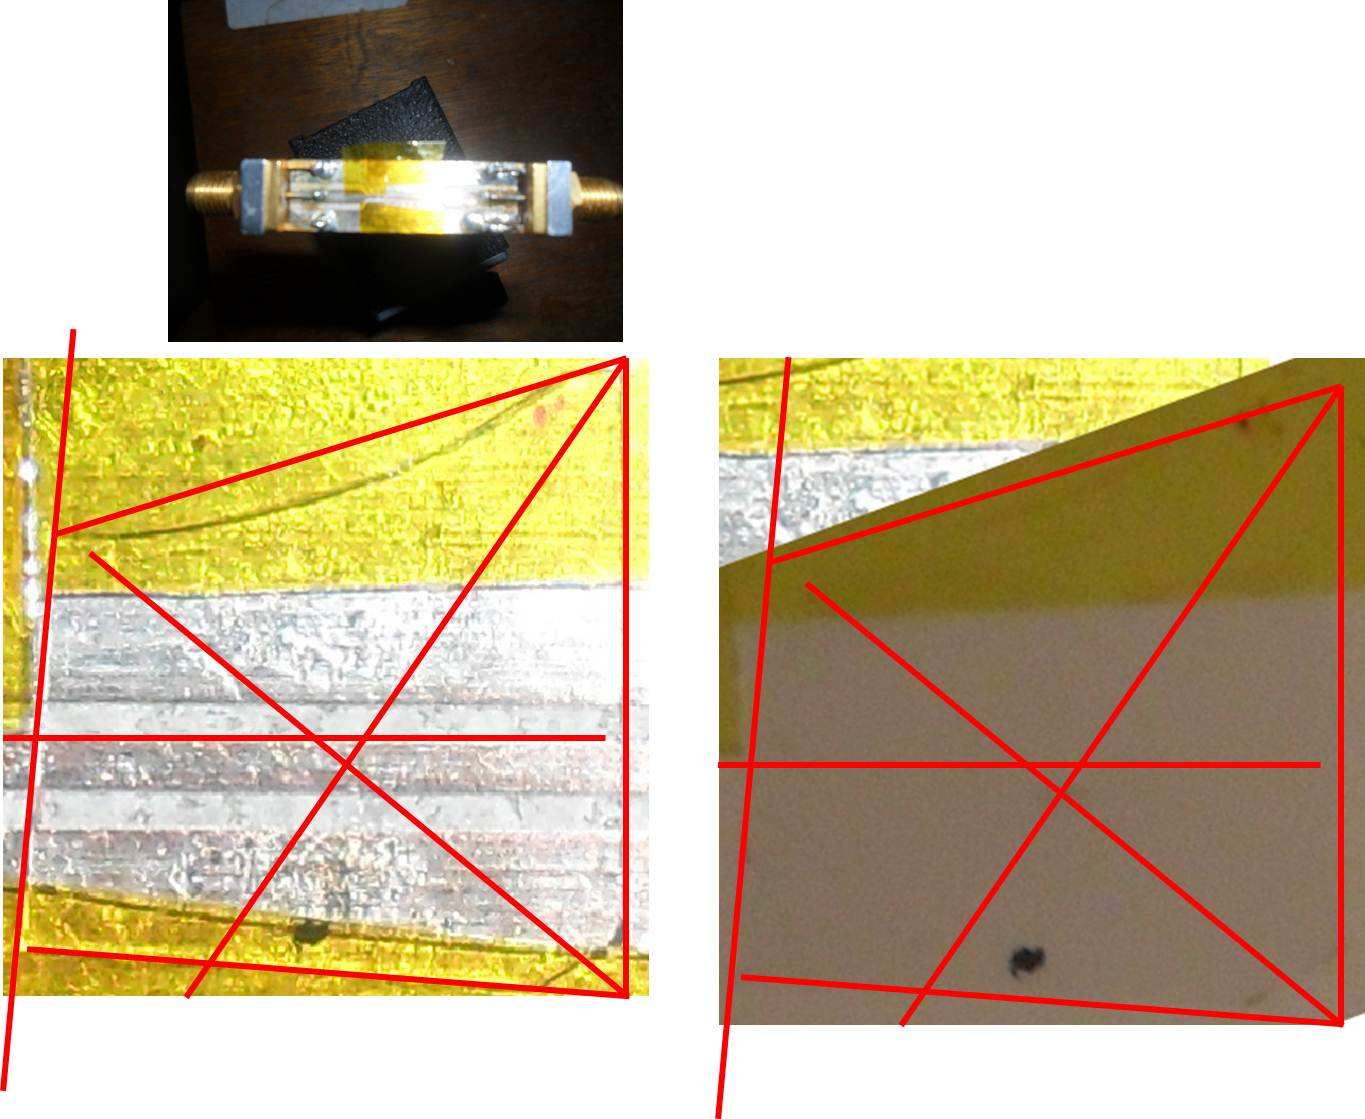
\includegraphics[width=0.8\textwidth]{PCB-Signal-line-Sample-Verification.jpg}

\caption{Using Microsfot Powerpoint, we can verify the sample lies on the signal line. We can see the sample in the left photo, but the scratches on the PCB make the sample invisible to the naked eye in the photo on the right. By making a series of reference points (here, we have used lines surrounding the glass), we can copy and paste this overlaying 'net', therefore showing the position of the sample relative to the PCB}
\label{overflow}
\end{figure}


With the sample now mounted on the PCB, the PCB can now be dropped on to the piezo-electric stage. After ensuring the magnetic ring is switched off, magnet (1) can be pulled out, breaking the circle. The piezo-electric stage can then be gently pulled towards the space left by magnet (1), and the sample merely dropped in to the slot at the centre of the stage. The two green cables, held in place either side of the stage by two clamps, can then be screwed on to the PCB. These two cables provide the electrical field with which we pump the structure.


\section{Setup alignment}

\section{Laser optimization}

\section{Optical alignment}
Optical alignment is the most important part of the experimental work and main condition of robust and repeatable measurements.

General advice:
\begin{itemize}
\item Follow the safety rules ALWAYS!!! You have two eyes only.
\item Use holders, screws and fasten optical components to the table. Firstly, it will prevent occasional movement of the component and disruption of alignment. Secodnly, all components are extremely expensive and one accidental falling of a mirror can cost hundreds of pounds.
\item Block and properly dump back reflections of filters and mirrors.
\item Check operating wavelength of mirrors. Make sure it fits your setup.
\item something else???   
\end{itemize}

\subsection{Delay line}
Delay line allows one to change length of optical path and introduce time delay between excitation of the investigated sample and moment of measurement.

% Links to a scheme is higly desirable.

Ideally the laser beam goes parallel to the rail of DL, incidents to the corner reflectors and reflects to the rotating mirror. Incident and reflected beams should be exactly parallel to each other. Otherwise, reflected beam walks up-down or left-right with DL movement and alignment of subsequent optical elements is impossible.   
 
\textbf{\underline{How to:}} 
\begin{enumerate}
\item Set DL to -300 mm position.
\item Install a screen before the corner reflector.
\item Using the directing mirror send the beam to the screen. The incident point should be over against left half of the reflector.
\item Remove the screen, install it somewhere near the directing mirror and catch spot of the reflected beam.
\item Using screws of the directing mirror, adjust position of the spot thus to make incident and reflected beams are roughly parallel.
\item Put a screen before the reflector and check where the beam goes to. If the incident beam is very close to the reflector's edge, move the directing mirror perpendicular to DL axis and fix it.
\item Repeat steps 4-5.
\item Install, connect and focus the CCD camera thus to see image of reflected spot on the TV screen.
\item Notice the spot position.
\item Open control panel of the DL
\item Make a small step of DL in positive direction (for instance, 10 mm).
\item Most likely, position of the spot will be changed. Rotate the direction mirror screws and set the spot in initial position.   
\item Repeat steps 11 and 12 till position of the spot depends on DL shift. If you achieve opposite end of the DL (+300 mm), move it to the origin (-300 mm) and continue alignment. If the incident beam is very close to the reflector's edge, move the directing mirror perpendicular to DL axis and fix it.
\item Install the rotating mirror to send the beam to the microscope.
\item Put the screen after the rotating mirror and repeat steps 8 - 13.
\end{enumerate}

 
\subsection{Microscope}


\section{Sample installation}

\section{Pulse measurement}

\section{CW measurement}


\subsection{Configuring the laser}

%The workings of the Tsunami laser system has been described well in the Doctoral Thesis presented by Toby Davison\footnote{url{https://eric.exeter.ac.uk/repository/handle/10036/3675}}. Here, I shall merely describe how to obtain an output laser beam, of wavelength 400nm. The mirror directly in front of the laser aperture should be raised, so as to protect the sample from the laser until it is configured correctly. The console next to the laser should display 'Standby'. This indicates, of course, the laser is on standby. Pressing and holding the upper-left button on the console switches the laser on, and now the power of the laser is displayed (initially this is '<0.1W'). Wait for around 2 minutes, until the laser outputs 12W. This is the maximum power of the laser, and we are now able to see the red laser beam reflected on to the card next to the laser aperture.

%Switch the Thorlabs S142C power meter on, and adjust the meter so that it measures in units of mW, and reads the intensity of 800nm (red) light. Place the power meter in between the mirror and the black card (so that it interrupts the red beam's path), and rotate the meter until the power incident is maximised. With reference to the order given in Figure 3, adjust the dials on top of the Tsunami Laser until the power recorded is maximised further. From experience, it is recommended that this step be repeated, as this this often provides a further maximisation. With the power now maximised, the power meter can be removed and put aside.

%\begin{figure}
%\includegraphics[width=0.8\textwidth]{Tsunami_Laser_System.jpg}
%\caption{Turn the dials in the order A, B, C and D, maximising the power measured.}
%\label{overflow}
%\end{figure}

%The oscilloscope above the bench-top should now be switched on. A peak near 800nm, and with a difference of around 10nm, should be readily seen (notice the bench-top should be relatively dark: ambient light will disrupt this reading). Turning the dials on the Tsunami system, labelled $\lambda$ and $\Delta$$\lambda$, will give us a laser beam of 800nm and difference of 13nm. With this setting in place, the frequency of the laser system now needs to be locked to the master clock. Our attention now shifts to the lock-to-clock system.


%The frequency on display should be oscillating significantly, around 0.001GHz. A fault has been identified: if this oscillation is not observed, switch the master-clock, the lock-to-clock device, and the photodiode box directly above the lock-to-clock box off. Switch these back on, in the order master-clock, photodiode box, and the lock-to-clock, and the frequency displayed should now be oscillating as expected. Using the up-down arrows, the frequency displayed should be adjusted so it oscillates around 80.00000GHz: once this is achieved, the button to the left of the display should be pressed, thus locking the frequency after around 5s. The laser is now fully operational.

%\subsection{Adjusting the laser beam path}

%Before we manipulate the path of the laser beam across the bench-top, place the silver stand just before the piece of tubing, situated next to the microscope. The mirror in front of the laser aperture can now be lowered, and the blue laser beam should be visible on the silver stand's white paper. If the spot profile is circular, no adjustments need to be made. If however the laser beam is not circular, or not visible at all, the path of the laser beam must be misaligned. To repair this, use a small piece of card to observe the laser beam before it reflects off each individual mirror, and then adjust the mirror accordingly. Obviously, we should intially check the mirror closest to the laser aperture, and then move on to the next one step by step. Best practise also dictates the laser beam should ideally be reflected off the centre of each mirror.


%An important consideration is the beam path when the retroreflector is moved. Place the power meter just in front of the silver stand, and configure it so it measures light of 400nm (blue) in mW. Rotate the meter until the incident intensity is a maximum. The power incident on the power meter, and therefore the power meter, can now be varied by roating the neutral density filter (situated after the delay line). {\bf The damage threshold of the photodectors is 4mW}: thus the optical filter should always be rotated such that the beam power is below 3.5mW, before allowing the laser beam to enter the microscope. By opening Internet Explorer, logging on to the url http://192.168.0.254, entering the position for the retroreflector to move to ($\pm$300mm are the limits), setting a velocity 20mm/s, and running the program, we can move the retroreflector from one end of the delay line to the other. After shifting the retroreflector, the laser beam ideally should neither move nor change in intensity. From experience, the laser beam intensity varies by up to 10% when the retroreflector is moved by 60cm, and this is attributed to diffraction.


%If however the beam moves, a more time-consuming procedure must be followed to correct this. The following procedure was written by Dr. Volodymyr Kruglyak.

%"Let us consider two positions (marked as 1 and 2) of the retroreflector on the translation stage (e.g. at the two opposite ends).

%\begin{figure}
%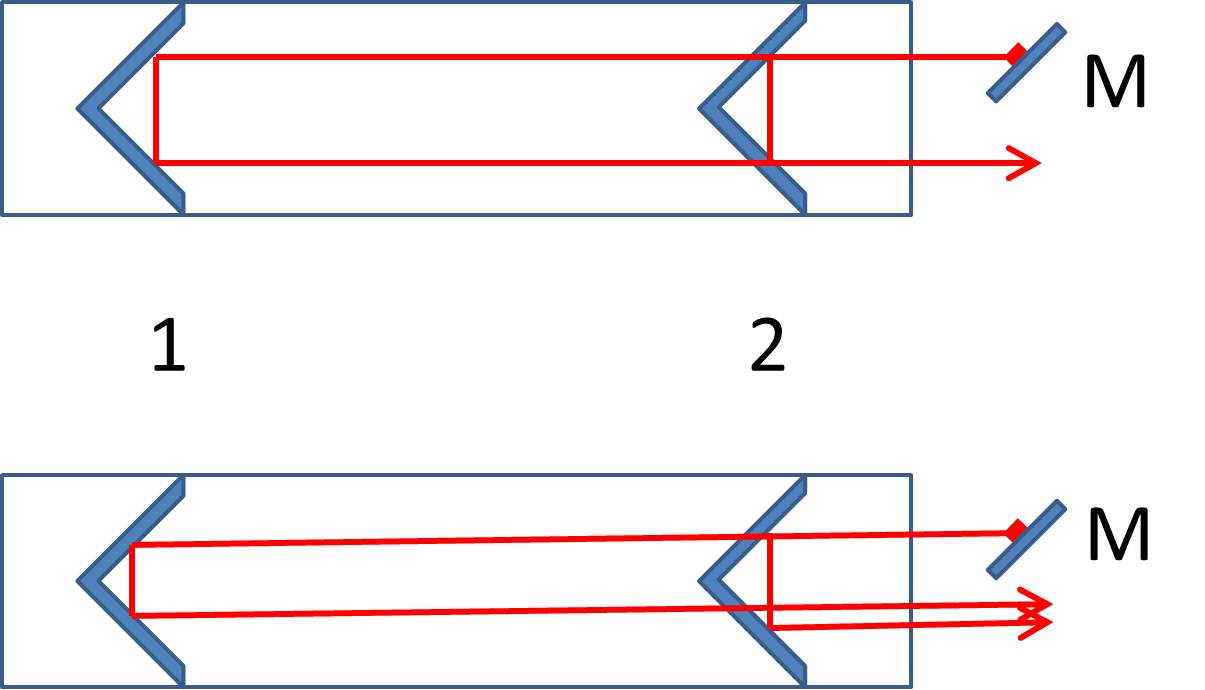
\includegraphics[width=0.8\textwidth]{Retroreflector.jpg}
%\label{overflow}
%\end{figure}

%The top sketch corresponds to a good alignment: the stage travel strictly parallel to the directions of the beams (it is the key property of the retro-reflector to send the incident beam exactly in the antiparallel direction), and so, the beam hits exactly the same points of the retroreflector in both positions.

%The bottom sketch illustrates what happens when the beam is slightly deviated from the direction of stage’s travel: the beam hits different points of the retroreflector in its different positions on the translation stage, and as a result, the beam gets translated as the stage travels.

%To fix this, you need to do the following: Assuming that the beam is translated away from the axis of the stage as it approaches the input mirror (“M”) – i.e. as shown on the bottom sketch, you need to adjust mirror M so as to deviate the beam even further from the axis when stage is in the furthest position from mirror M."

%\subsection{Positioning the sample/Focussing the laser beam}

%With the laser beam still blocked, the piezo-electric stage can be moved so that the PCB lies directly underneath the objective lens. Open the program "PI Mikromove", and follow these steps:

%\begin{enumerate}
%\item Highlight the top option displayed, click 'connect', and then 'ok'
%\item Press 'negative Limit', and then 'start'
%\item Wait a few seconds until the program has finished running, and then press %'close'
%\item In the new window that has opened, open the tab 'connections', and click 'new'
%\item Highlight the remaining axis, and click 'connect'
%\item Click 'ok', press 'negative limit', 'start', wait until the program stops, and then 'close'
%\end{enumerate}

%The window that has now opened displays the two axes. Change the step size on both axes to 3mm, and then incrementally move the PCB to 21mm x 21mm. This has centred the PCB.

%We also need to centre the objective lens. Open the program 'Measurement \& Automation Explorer', and double-click "devices" on the left panel. Right click 'device 0' or '1', and communicate with the instrument. We want to communicate with GPIB 15. In this panel, type:

%\begin{itemize}
%\item Typing '1TP', '2TP' or '3TP' then pressing 'query' returns the position of the PCB in the x-,y- and z- axes.
%\item Typing '1MAxxx', '2MAxxx' or '3MAxxx', where xxx is a co-ordinate in $\mu$m, and pressing 'write' moves the PCB to the appropiate co-ordinate in the x-, y- or z- axes.
%\end{itemize}

%Move the objective lens such that it lies directly above the top of the PCB ie. write the commands '1MA150' and '2MA150'.

%We now need to focus the sample. Allow the laser beam to enter the TRSKM apparatus, and push the mirror in between the PCB and the objective lens. With your hands below magnet 1 (which is still pulled out of the circle), carefully raise the PCB towards the objective lens using your left hand. Do not push the PCB in any transverse or longitudinal direction. Once the laser beam is reflected on to the piece of card, such that there are 2 dots visible, carefully raise or lower the PCB until the 2nd dot is strongly concentrated, and use your right hand to turn the dial under the PCB to tighten its position. Switch the tv on next to the display monitor, and you should be able to see a rough surface. If not, again raise or lower the sample until you can see the PCB board in focus on the CCTV monitor.

%Open the window 'PI Mikromove', and now, in increments of 20$\mu$m, move the piezo-electric stage until the structure can be seen on the CCTV monitor. This is mainly done through trial and error. The CCTV monitor can now be switched off, and the mirror above the PCB can be pulled out. The laser beam is now entering the objective lens, and is being collected by the photodetectors.

%\subsection{Taking a reflectivity scan}

%\begin{figure}
%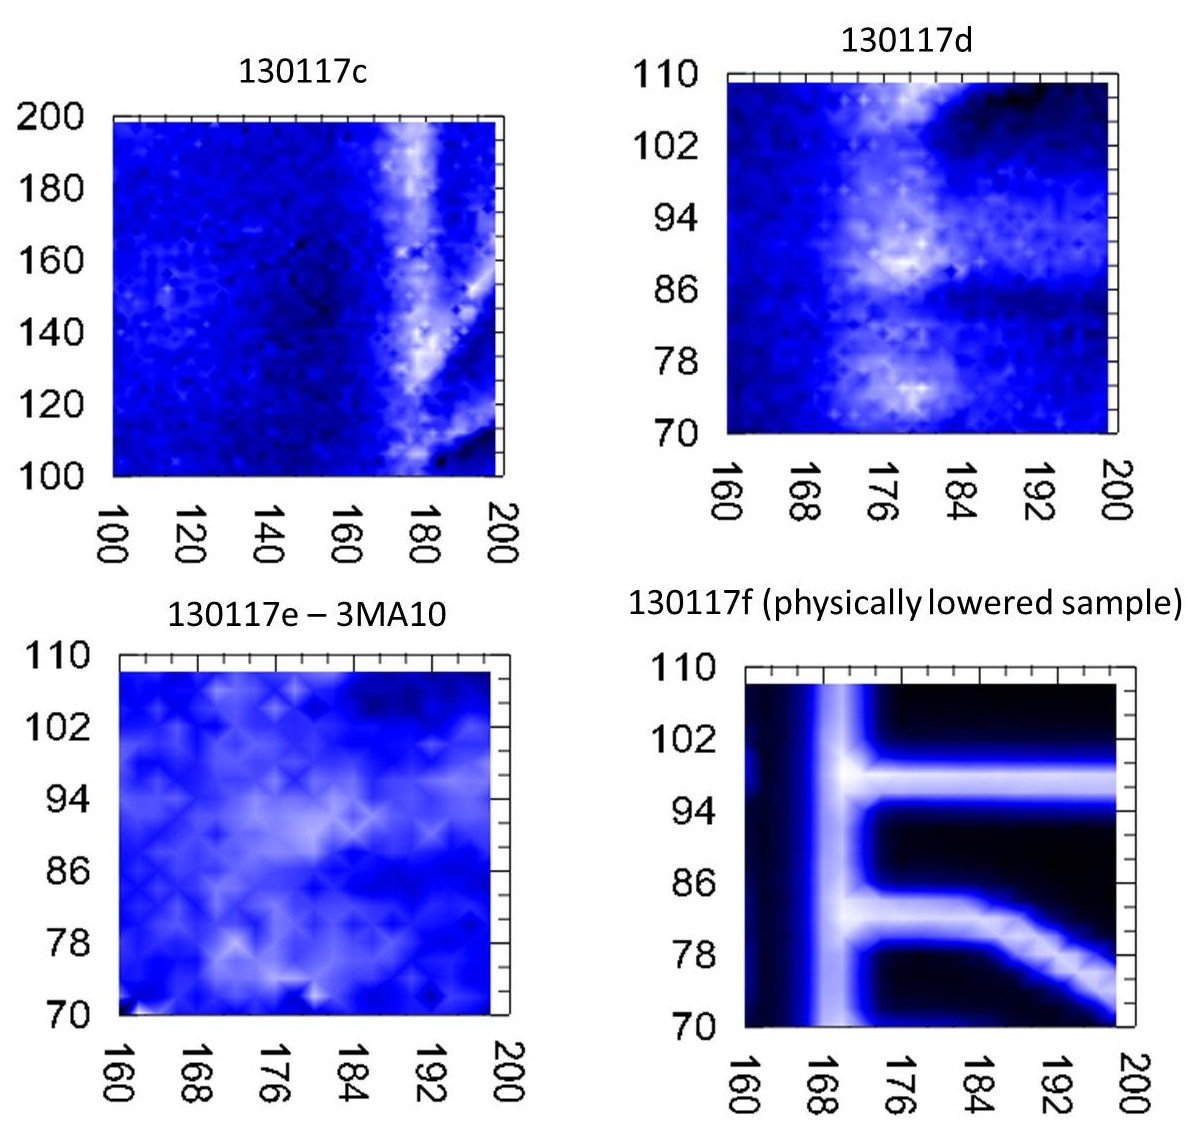
\includegraphics[height=3in]{Reflectivity_Scan.jpg}
%\caption{Example reflectivity scans, showing the effect of adjusting the focus, and therefore letting us obtain a focussed image}
%\label{overflow}
%\end{figure}

%We must firstly ensure the laser beam is focussed when entering the photodiodes. Open the LabView windows 'simple voltmeter AI3' and 'simple voltmeter AI7'. Run AI7's screen, with the laser beam blocked, and the voltage shown should be constant (at the time of writing, it has always been -0.0067V). Similarly, AI3 should also be constant (at the moment, -0.0082V). If the voltage is oscillating, some wires have been switched: please refer to figure 8 to repair this. Now unblock the laser beam, and turn the four dials within the bridge detector, maximising the voltage on screen. We are aiming to obtain the greatest change in the intensity of the reflected beam, when the laser beam moves on to and off the permalloy sample.

%Open the LabView window "probe station imaging 110606". Enter 0 to 300$\mu$m in the forms for the start and end of the scan in the x- and y- axes, and make the step size around 3 $\mu$m (thus making the step number 300/3 = 100 in both directions). Now run the scan, ensuring the bench is in darkness.Once the scan is complete, the structure should be visible. Now we can zoom in on certain areas, obtaining an improved image of the structure, and the focus can be further improved, using "PI Mikromove's" 3MA command to move the objective lens.
%\newpage

%\section{Applying a Pulsed Excitation}

%TRSKM can be used to experimentally determine the frequency response of a sample. A series of electrical pulses are applied across the PCB, thus exciting a range of frequency responses within the structure. A synchronised laser beam is then focussed on to the sample, and using the Magneto-Optical Kerr Effect, the change in magnetization is detected. The variation in magnetization with respect to time is found using a retroreflector mounted on a delay line. As the retroreflector moves, the path of the laser beam varies, causing the incident probing laser beam to detect the frequency response at different points in time. Depending on the sample's dimensions and physical properties, the frequency of ferromagnetic resonance (FMR) can therefore be found, by applying a Fast Fourier Transform to the time-varying data.

%\subsection{Constructing a pulsed electric field}

%To obtain a reflectivity scan, we have used solely the probing beam. To progress, we therefore now need to add an electric current to the system, to introduce a pumping mechanism. We will firstly look at the Picosecond Impulse Generator. Connect the green 'input' cable, from the PCB, to the 'impulse output' port. Secondly, attach a T-junction to the 'Gate Input' port, and connect one lead, from this, to the 'Ext 1' port on the oscilloscope, and the other to the function generator's 'sync' port. Thirdly, attach another cable between the 'clock input' port to the 80MHz output (+5dBm)' port of the master clock.

%The master clock regulates the synchronisation between all the different devices interacting in this experiment. We are concerned with three ports, as shown in Figure 5.

%\begin{figure}
%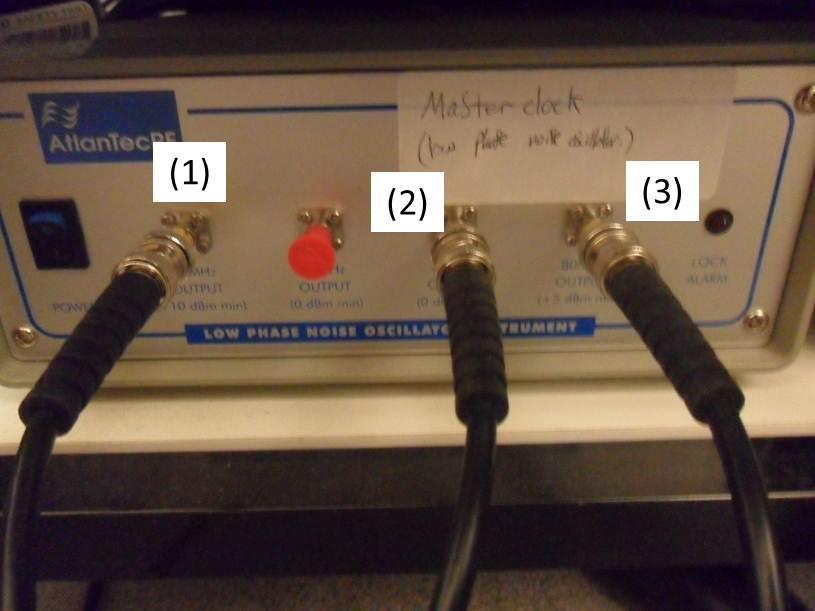
\includegraphics[height=3in]{Master_clock.jpg}
%\caption{The front of the master clock. {\bf (1)} Connected to the 'Ref In' port behind the continuous wave generator. {\bf (2)} Connected to the 'Ref In' port behind the 'Lock-to-Clock' box. {\bf (3)} Connected to the 'clock input' port on the Picosecond impulse generator}
%\label{overflow}
%\end{figure}

%The function generator should now be configured to generate a square wave, with a frequency of 3kHz. Switch the 33120A function generator on, and use the manual\footnote{\url{http://www.hit.bme.hu/papay/edu/Lab/33120A_Tutorial.pdf}} to generate such a wave.

%\begin{figure}
%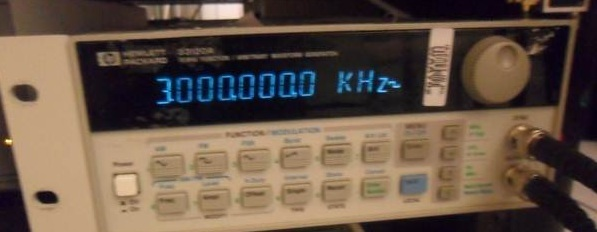
\includegraphics[height=2in, width=5in]{Function_generator.jpg}
%\caption{The display on the front of the function generator, when the function generator is configured correctly.}
%\label{overflow}
%\end{figure}

%The Lock-In Amplifier (LIA) is designed to reduce the amplitude of the noise in the signal. It can also collect different forms of the signal, but these are not essential for us to collect. Connect a cable between the function generator's 'output' port and the LIA's 'Ref in' port. Now we must also connect port 'A' on the LIA's front panel to the 'RF Output' connected to the bridge detector.

%\begin{figure}
%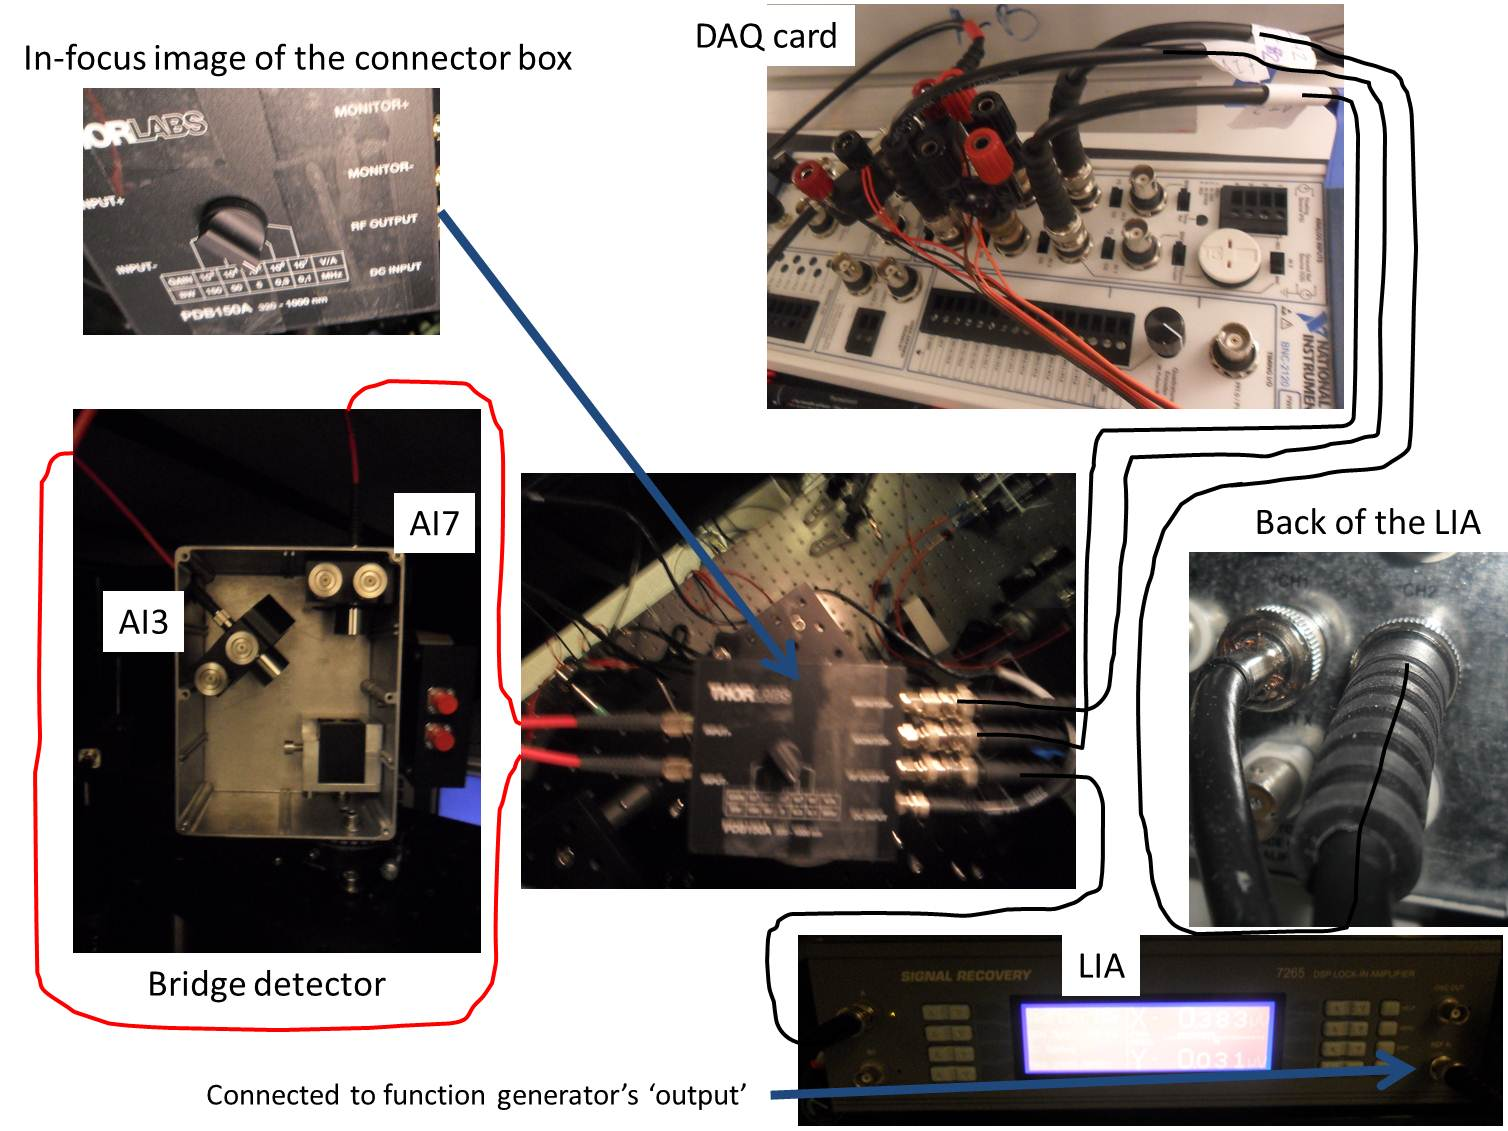
\includegraphics[height=3in]{Wiring_Network_Bridge.jpg}
%\caption{The connections between the LIA, the output from the bridge detector, and %the DAQ card}
%\label{overflow}
%\end{figure}

%Connect the green 'output' cabe from the PCB to the 'Ext 2' port on the oscilloscope. There is now a complete circuit connected to the PCB, and so switching the Picosecond Generator on will generate a pulsed electrical current, and therefore a pulsed field.

%\subsection{Applying an external magnetic field}

%\begin{figure}
%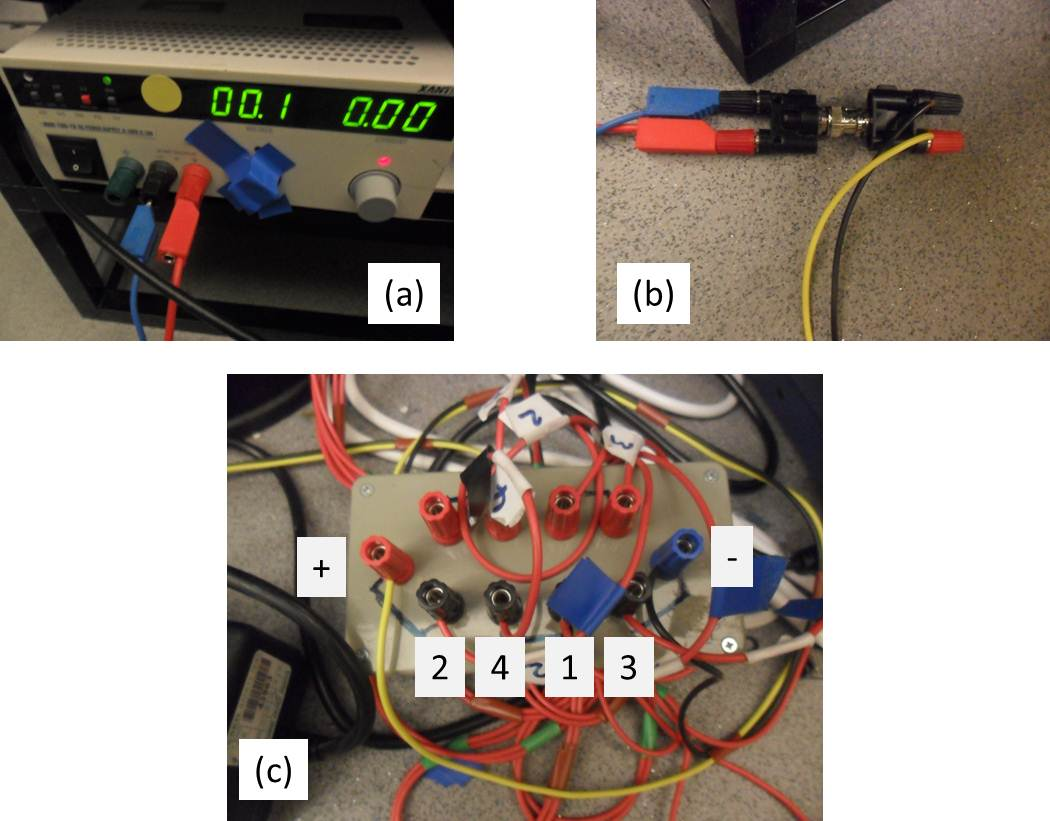
\includegraphics[height=3in]{Magnetic_wiring.jpg}
%\caption{The wiring associated with the connector box connected to the quadruple magnets {\bf (a)} The front of the magnetic field generator. {\bf (b)} The connection between the two plugging wires in (a) and the + and - connectors in (c). {\bf (c} The order in which the quadrupoles are connected to the box, in order to generate a magnetic field parallel to the PCB}
%\label{overflow}
%\end{figure}

%Now that we are applying a pulsed current through the PCB, we need to apply an external magnetic field across the sample. Ensure the four quadrupole magnets are in a complete unbroken circle, and connected to the connector box. The connection should be in the order given in the figure below.

%Switch the box shown in Figure 8 (a) on. Open the Labview window 'gen voltage update - copy.vi'. In the 'Channel Parameters' section, select 'Dev2/Ao0', and enter 0.200V in to the form directly underneath 'Voltage Output'. Now hit run. We can monitor the magnetic field in real time by running the Labview window 'hall generator double on pole 110523.vi' simultaneously. Incrementally increase the voltage, running after increasing the voltage by 0.2V, until we have a voltage output of 1.2V. For permalloy, this is sufficiently above the magnetisation of saturation. Now reduce the voltage, until the desired magnetic field as seen in 'hall generator double on pole 110523.vi' is obtained.

%\subsection{Taking a pulsed scan}

%We now need to move the laser spot to the appropiate co-ordinates incident on the sample. This could potentially be done through using 'PI Mikromove', to move the sample stage, but to increase speed, we will instead move the laser spot. After taking a reflectivity scan, as described in chapter 1, we should know the position at which we want the laser to hit the sample. Thus open the Labview window 'move laser spot in rotated coordinates.vi', and enter the position at which we want to measure the magnetic response of the sample.

%We are now ready to take an optical delay scan of the sample. Open the Labview program 'yatyin probe station optical delay scan 111125.vi', and enter -300mm to +300mm in the start and finish columns. The step size can vary: for a quick scan, we can use 1-2mm, but for results which you will want to take a FFT of, a delay step of 0.5mm is needed. 1500ms to wait is optimal (this should, as a general rule of thumb, be 3 times larger than the time constant). Tick the predefined file name button, and enter, in the form 'Kerr rotation', the folder in which you would like to store your scan. Now press run. 

%\begin{figure}
%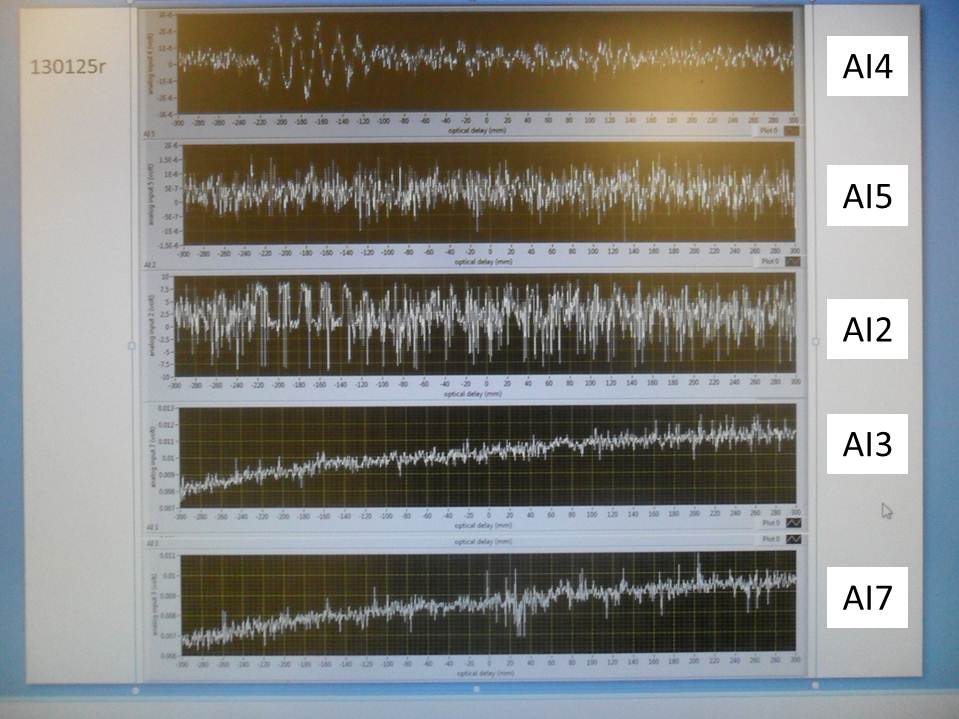
\includegraphics[height=3in]{Pulse_scan.jpg}
%\caption{A typical scan, showing a pulsed excitation. The oscillations in the signal %AI4 clearly show there is a pulsed scan running.}
%\label{overflow}
%\end{figure}

%The retroreflector will take a little time to start (under a minute), and now you will need to wait for the optical delay scan to complete. Once the scan is complete (ie you can see a full graph ranging from -300mm to +300mm for AI4 on screen), a  window will appear, asking for the name with which to save the file. Generally, best practice suggests using a filename 'yymmdda.txt', where yymmdd is the date, and a is the first scan of the day. When this is saved, another window will ask for the filename of the image parameters of the scan we just ran - use 'yymmdda-i.txt' for this second file.

%The data of interest, collected from this scan, will be stored in the 'yymmdda.txt' file. To take a Fast Fourier Transform of this signal, to identify the resonant frequency, follow the instructions described in appendix A.
%\newpage

%\section{Applying a Continuous Wave (cw) Excitation}

%From chapter 2, we have deduced the resonant frequency of an antennae $\omega_r$. Our experimental setup of TRSKM exploits a dispersion mismatch, arising due to the coupling of two different geometries, such that the excitation of ferro-magnetic resonance (FMR) in one structure injects spin waves, of finite wavevector, in to the second geometry. If we therefore apply a continuous wave excitation, of frequency $\omega_r$, we will observe the injection of spin waves in to the waveguides coupled with the antennae.

%\subsection{Switching the pulsed current to a continuous one}

%For ease, I shall assume the bench-top is in the configuration ready to gather pulsed scans. We merely therefore need to simply switch the Picosecond impulse generator for a continuous wave generator. Switch the impulse generator off, remove the green cable from the 'impulse output' port, and cap the port. Move this green cable to the 'RF 50$\Omega$' port on the front panel of the continuous wave generator. Disconnect the T-junction from the 'gate input' port, and replace the T-junction with a linear connector. Remove the non-green cable connected to the oscilloscope ('Ext 1'), and connect this lead to the 'Pulse In' port on the continuous wave generator. Now switch the continuous wave generator on. We have now replaced the pulse generator with a cw generator.

%\subsection{Running the cw scan}

%The procedure needed to collect dynamical scans is automated. Thus, after configuring several LabView windows, the system can be left alone, and we only need to wait for the data to be collected. Apply an appropriate magnetic field across the sample, and open the Labview window 'yatyin probe station imaging 110606a.vi'. Conduct a reflectivity scan as normal. Once the reflectivity scan is complete, and you are happy with the focus on-screen, tick the cursors so that AI4 is acquired, and the filename is predefined. Now minimise this program.

%Open the LabView window 'SMF100A controller.vi'. We want to use a frequency which is as close to the frequency of FMR of the antennae as possible, but is also a multiple of 80MHz. For example, if the FMR frequency were 7.5GHz, we would use a continuous wave frequency of 7.52GHz. Therefore enter the desired frequency in the form, and enter a power of 22dBm. Tick 'pulse modulation' then run, and then tick 'RF', then run. The display on the continuous wave generator should now show these two parameters. If an error occurs, try closing all the LabView windows, then reopen. This repaired the only problem we encoutered with this stage. We can now minimise this window.

%Open the Labview window 'generate optical delays.vi'. Enter the frequency we have already decided, and enter the delays you want to use. Typical delay values are -36mm to -18.5mm, where the delay interval is 2.5mm. This is sufficient to map the propagation of several spin waves. Enter the first delay position, as indicated, and run this program. An example of this completed window is given in figure 11. Now we can minimise this window.

%\begin{figure}
%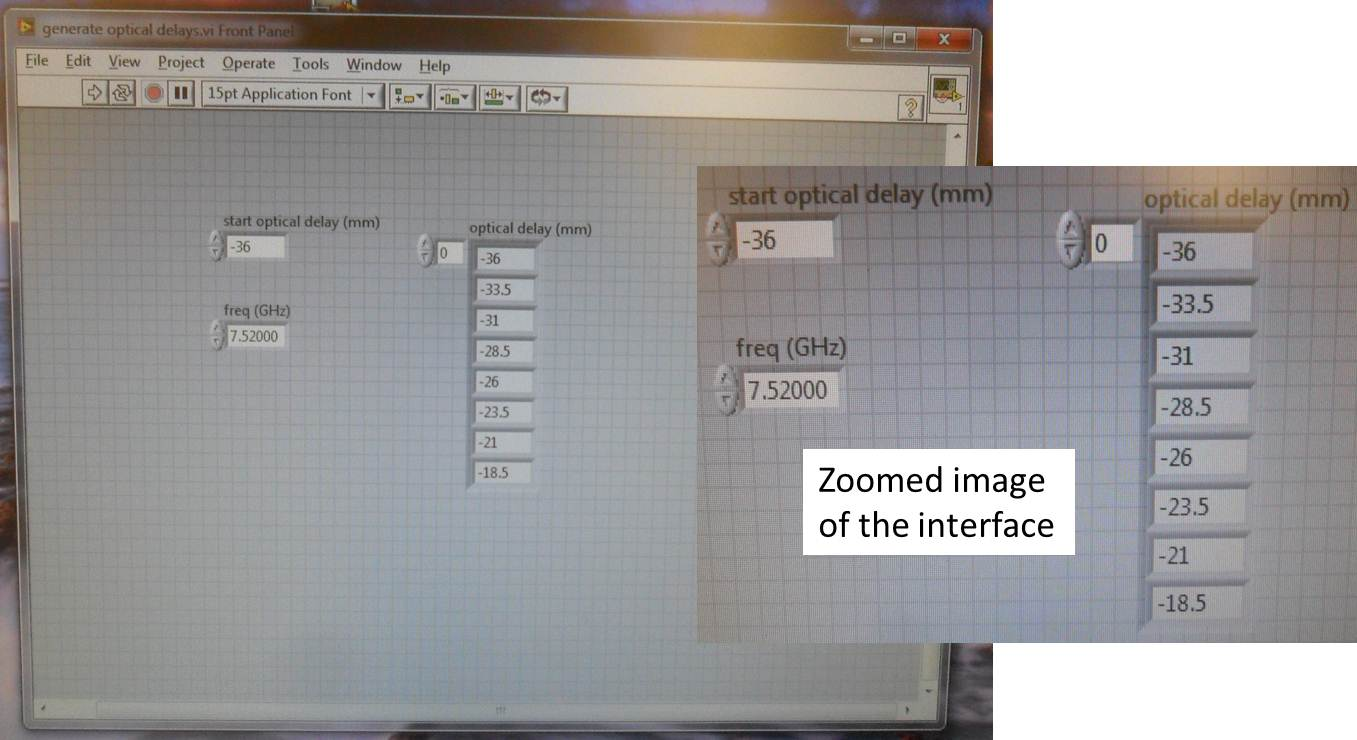
\includegraphics[height=3in]{ODs_window.jpg}
%\caption{An example of a completed 'Multiple Kerr Imaging 110606a.vi' window}
%\label{overflow}
%\end{figure}

%Now open the LabView window 'Multiple Kerr Imaging 110606a.vi', and enter the scan parameters as desired in to the ten forms on the left. Create a folder in which you would like to store the files acquired from the scan, and enter the path name (only folders go here: no text files etc should be referred to) in to the lower form. In the 2 colums on the right, enter the dealys, and the appropriate filenames. An example of this window can be seen in the figure below. Run this program, and now just leave the bench-top in darkness for the time-resolved scans to assimilate.

%\begin{figure}
%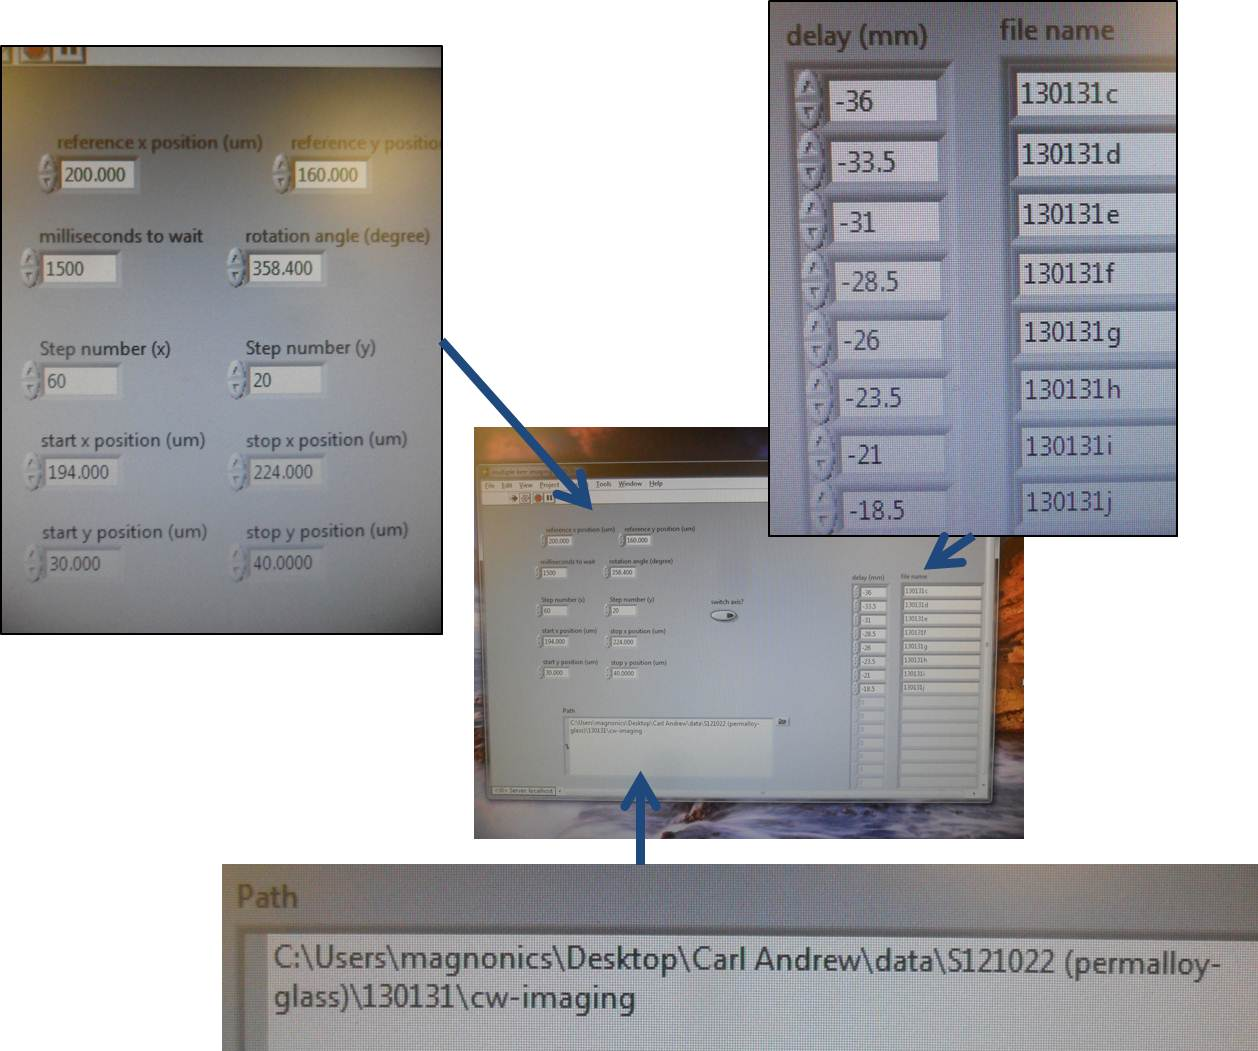
\includegraphics[height=3in]{MKI_window.jpg}
%\caption{An example of a completed 'Multiple Kerr Imaging 110606a.vi' window}
%\label{overflow}
%\end{figure}

%When the scan has finished, use the procedure described in Appendix B to acquire %static and dynamical images of the data obtained.
%\\

%Notice the laser usually stops working after around 36 hours of running continuously: this is usually due to natural overheating. The PCB also drifts, due to natural disturbances, and deactivating the laser system obviously deactivates the laser. All these are hazards with running the continuous images, and therefore regular checks should be made, whilst the scans are running, to check everything is running smoothly.
%\newpage

\end{document}